\subsection{The Kruskal extension \checkmark (still questions)}
		\begin{figure}[htbp]
			\begin{center}
				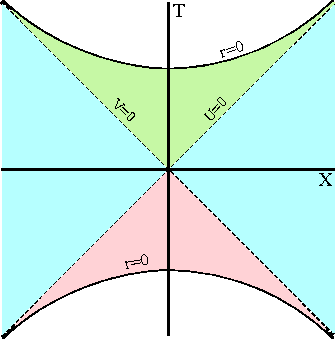
\includegraphics[scale=1]{kruskal}
			\end{center}
			\caption{This is the $XT$ plane of the \textbf{Kruskal extension}. The horizons are the dashed lines. The {\color{blue} blue} wedges are the exterior, the {\color{forestgreen} green} wedge is the future interior and the past interior is in {\color{red} red}. Nothing can escape the {\color{forestgreen} green} wedge into the {\color{blue} blue} wedges, because there is no radial null geodesic which would connect the wedges.}\label{kruskal}	
		\end{figure}
	From here on, we will use $r_{s}=2GM=1$.\footnote{This means, the Schwarzschild geometry looks like $\diff s^2=-\frac{r-1}{r} \diff t^2+\frac{r}{r-1}
		\diff r^2+r^2 \left( \diff \theta^2+\sin^2\theta \diff \phi^2 \right)$}
	Instead of using the coordinates $(t,r,\Omega)$ like in the previous section, we now introduce the Kruskal-Szekeres coordinates, because they are a better choice for near-horizon physics.
	
	First we parametrize the radial null geodesics in the Schwarzschild geometry as
		\begin{equation}
			t=\pm r_{*} + C,
		\end{equation}
	where C is some constant of motion and $r_{*}$ is a new radial coordinate defined as
		\begin{equation} \label{r_*tortoise}
			r_{*}\equiv r+\log (r-1).
		\end{equation}
	also called the \textit{tortoise coordinate}\footnote{The name \textit{"tortoise"} has its origin in the paradox of Achilles and the tortoise.}, because now we have an infinite coordinate range that fits in a finite geodesic distance.
		
	The Kruskal-Szekeres coordinates are then defined as
		\begin{equation}
			U\equiv -e^{\frac{r_*-t}{2}} \label{U}
		\end{equation}
		\begin{equation}
			V\equiv e^{\frac{r_*+t}{2}}.
		\end{equation}
	%\clearpage			%vllt mal Marei fragen, wie man das besser mit den footnotes machen kann
	Their lines of constant U and V are radial null geodesics and these coordinates have the property, that
		\begin{equation}
			 UV=(1-r)e^r.
		\end{equation}
	This means we have a singularity at $UV=1$ and the horizon is at $U=0$ or $V=0$. The metric looks now like
		\begin{equation}
			\diff s^2=-\frac{2}{r}e^{-r}\left(\diff U \diff V + \diff V \diff U\right)+r^2 \diff \Omega^2_{2}
		\end{equation}
	Because this metric still has an off-diagonal tensor, we define another set of coordinates
		\begin{equation}
		\begin{split}
			U=T-X 	\\	
			V=T+X
		\end{split}
		\end{equation}
	Now the metric looks as follows:
		\begin{equation}\label{SchXT}
			\diff s^2=\frac{4}{r}e^{-r}\left(- \diff T^2+ \diff X^2\right)+r^2 \diff \Omega^2_2
		\end{equation}
	Note that there is now no singularity at $r=1$.
	
	This metric defines a geometry over the full XT plane, which can be seen in Figure \ref{kruskal}. The \textbf{right {\color{blue} blue} wedge} is, in the old Schwarzschild coordinates, former $r>1,~-\infty<t<\infty$. If one wants to continue to $r<1$, there is a branch cut \marginpar{wie sieht dieser branch cut genau aus?} defined in \eqref{U}, which allows us to either go to the regions with $X^2-T^2<0$ and $T>0$ which is the \textbf{{\color{forestgreen} green} wedge}, or the \textbf{{\color{red} red} wedge} with $T<0$ and also $X^2-T^2<0$. At last we have the left {\color{blue} blue} wedge in which we also can have $r\gg1$. Both blue wedges are asymptotically Minkowski regions. 
	
	The singularity $r=0$, which you find at the top and the bottom of \textbf{Figure \ref{kruskal}}, is the hyperboloid $X^2-T^2=-1$. It has two connected components, one at each boundary of the {\color{forestgreen} green} and the {\color{red} red} regions. These two regions are also called the {\color{forestgreen} future} and the {\color{red} past} interiors, while the other two are called the original/new exteriors (right/left {\color{blue} blue} wedges).
	
	All regions together can interpret the full Schwarzschild metric as a wormhole connecting two nearly flat universes, both acting at $r\gg1$ as if there were a point source of mass $M$. Signals can not travel through the wormhole, but two observers coming from opposite sides could meet in the middle and compare notes. \marginpar{how the hell does he know that?}